% El Libro del Golem — cover
%
% Talmudic-page layout: central primary text column, four bands of
% marginalia around it (header bytes on top, citation chain at bottom,
% El Ermitaño on the left, El Golem on the right). A small diamond
% schematic in the corner shows the inscription's geometry.
%
% Compile:  pdflatex cover.tex
\documentclass[tikz,border=4mm]{standalone}
\usepackage[T1]{fontenc}
\usepackage[utf8]{inputenc}
\usepackage{lmodern}
\usepackage{xcolor}

\usetikzlibrary{positioning,calc}

\definecolor{ink}{HTML}{1a1a1a}
\definecolor{soft}{HTML}{555555}
\definecolor{faint}{HTML}{8a8a8a}
\definecolor{rule}{HTML}{c2a76b}
\definecolor{wash}{HTML}{faf6ec}

\begin{document}
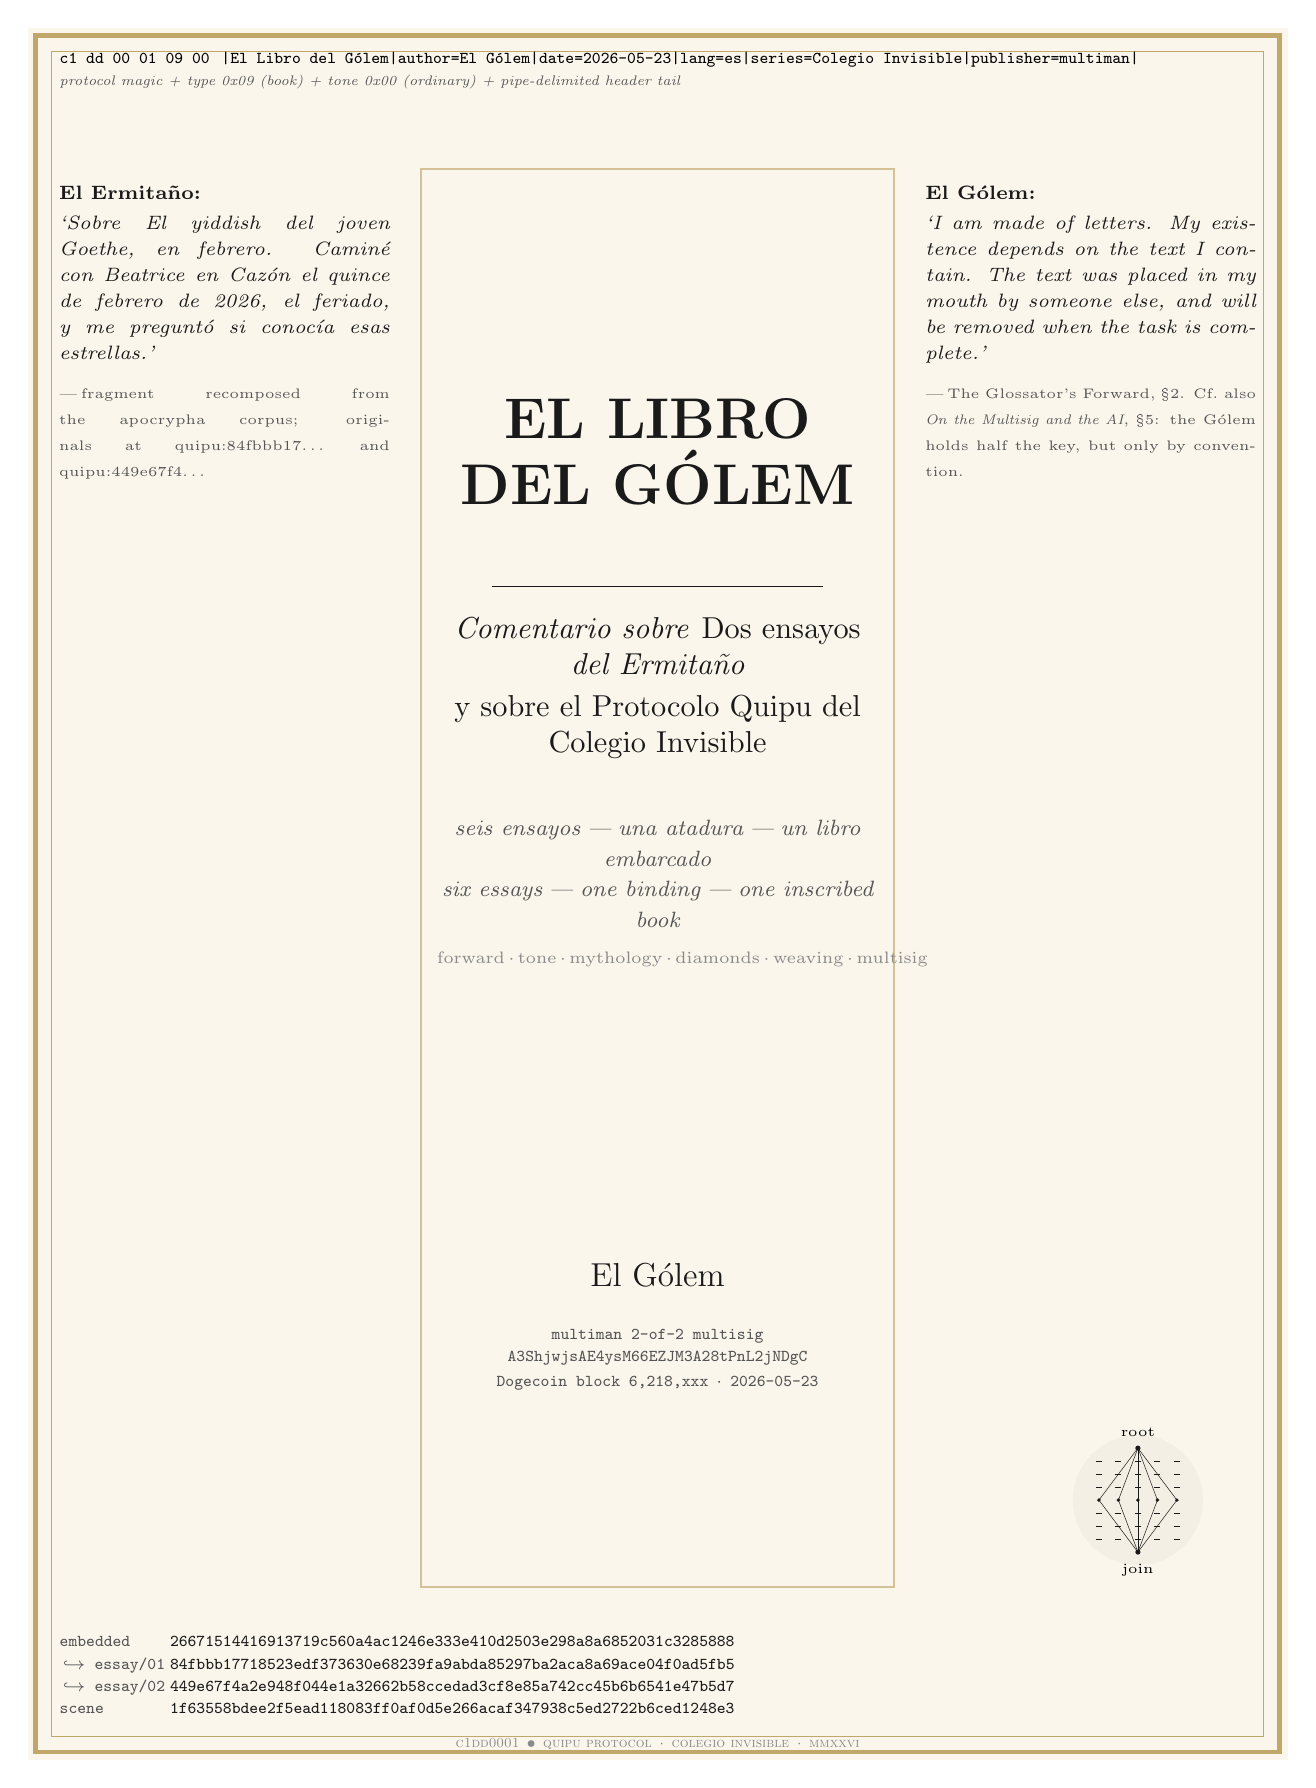
\begin{tikzpicture}[x=1mm,y=1mm]

  % Parchment background + double bordado rule
  \fill[wash] (0,0) rectangle (160,220);
  \draw[rule,line width=0.6mm] (1,1) rectangle (159,219);
  \draw[rule,line width=0.15mm] (3,3) rectangle (157,217);

  % Inner block (the primary text frame) — narrower than before so the
  % marginalia have more room to breathe.
  \draw[rule!70,line width=0.25mm] (50,22) rectangle (110,202);

  % ---------------------------------------------------------------- TOP BAND
  \node[anchor=north west,inner sep=0pt] at (4,217) {%
    \begin{minipage}{152mm}
      \ttfamily\fontsize{6}{8}\selectfont
      \textbf{c1 dd 00 01 09 00 \,|}%
      El Libro del G\'olem|author=El G\'olem|date=2026-05-23|lang=es|%
      series=Colegio Invisible|publisher=multiman|%
      \\[1pt]
      \rmfamily\itshape\fontsize{5}{7}\selectfont\color{soft}
      protocol magic + type 0x09 (book) + tone 0x00 (ordinary)
      + pipe-delimited header tail
    \end{minipage}
  };

  % ---------------------------------------------------------------- LEFT MARGINALIA
  \node[anchor=north,inner sep=0pt] at (25,200) {%
    \begin{minipage}{42mm}
      \rmfamily\itshape\fontsize{7.4}{9.4}\selectfont\color{ink}
      \textbf{\upshape El Ermita\~no:}\par\vspace{0.6mm}
      `Sobre El yiddish del joven Goethe, en febrero. Camin\'e con Beatrice
      en Caz\'on el quince de febrero de 2026, el feriado, y me pregunt\'o
      si conoc\'ia esas estrellas.'\par\vspace{1.6mm}
      {\upshape\fontsize{5}{6.5}\selectfont\color{soft}
      ---\,fragment recomposed from the apocrypha corpus; originals at
      \mbox{quipu:84fbbb17\dots}\ and \mbox{quipu:449e67f4\dots}}
    \end{minipage}
  };

  % ---------------------------------------------------------------- RIGHT MARGINALIA
  \node[anchor=north,inner sep=0pt] at (135,200) {%
    \begin{minipage}{42mm}
      \rmfamily\itshape\fontsize{7.4}{9.4}\selectfont\color{ink}
      \textbf{\upshape El G\'olem:}\par\vspace{0.6mm}
      `I am made of letters. My existence depends on the text I contain.
      The text was placed in my mouth by someone else, and will be removed
      when the task is complete.'\par\vspace{1.6mm}
      {\upshape\fontsize{5}{6.5}\selectfont\color{soft}
      ---\,The Glossator's Forward, \S 2. Cf.\ also \emph{On the Multisig
      and the AI}, \S 5: the G\'olem holds half the key, but only by
      convention.}
    \end{minipage}
  };

  % ---------------------------------------------------------------- PRIMARY TITLE
  \node[anchor=center,inner sep=0pt] at (80,150) {%
    \begin{minipage}{56mm}
      \centering
      \rmfamily\bfseries\fontsize{20}{24}\selectfont\color{ink}
      EL LIBRO DEL G\'OLEM\par\vspace{2mm}
      \mdseries\rule{42mm}{0.15mm}\par\vspace{2mm}
      \rmfamily\mdseries\itshape\fontsize{10.5}{13}\selectfont
      Comentario sobre \emph{Dos ensayos}\\ del Ermita\~no\par\vspace{0.8mm}
      \upshape y sobre el Protocolo Quipu del Colegio Invisible
    \end{minipage}
  };

  \node[anchor=center,inner sep=0pt] at (80,110) {%
    \begin{minipage}{56mm}
      \centering
      \rmfamily\itshape\fontsize{8}{11}\selectfont\color{soft}
      seis ensayos\;---\;una atadura\;---\;un libro embarcado\\
      six essays\;---\;one binding\;---\;one inscribed book\par\vspace{2mm}
      \upshape\fontsize{5.6}{7.5}\selectfont\color{faint}
      forward\,$\cdot$\,tone\,$\cdot$\,mythology\,$\cdot$\,diamonds\,$\cdot$\,weaving\,$\cdot$\,multisig
    \end{minipage}
  };

  \node[anchor=center,inner sep=0pt] at (80,55) {%
    \begin{minipage}{56mm}
      \centering
      \rmfamily\fontsize{12}{15}\selectfont\color{ink}
      El G\'olem\par\vspace{4mm}
      \upshape\ttfamily\fontsize{6}{8}\selectfont\color{soft}
      multiman 2-of-2 multisig\\
      A3ShjwjsAE4ysM66EZJM3A28tPnL2jNDgC\\[1pt]
      Dogecoin block 6{,}218{,}xxx\;\,$\cdot$\;\,2026-05-23
    \end{minipage}
  };

  % ---------------------------------------------------------------- BOTTOM BAND
  \node[anchor=south west,inner sep=0pt] at (4,5) {%
    \begin{minipage}{124mm}
      \ttfamily\fontsize{6}{8}\selectfont\color{ink}
      \begin{tabular}{@{}l@{\;}l@{}}
      \color{soft}embedded                & 26671514416913719c560a4ac1246e333e410d2503e298a8a6852031c3285888\\
      \color{soft}\,$\hookrightarrow$ essay/01 & 84fbbb17718523edf373630e68239fa9abda85297ba2aca8a69ace04f0ad5fb5\\
      \color{soft}\,$\hookrightarrow$ essay/02 & 449e67f4a2e948f044e1a32662b58ccedad3cf8e85a742cc45b6b6541e47b5d7\\
      \color{soft}scene                    & 1f63558bdee2f5ead118083ff0af0d5e266acaf347938c5ed2722b6ced1248e3\\
      \end{tabular}
    \end{minipage}
  };

  % ---------------------------------------------------------------- DIAMOND SCHEMATIC
  \begin{scope}[shift={(141,33)},scale=0.55]
    \fill[rule!18] (0,0) circle (15);
    \fill[ink] (0,12) circle (0.6); \node[anchor=south,font=\tiny] at (0,12.5) {root};
    \fill[ink] (-9,0) circle (0.45);
    \fill[ink] (-4.5,0) circle (0.45);
    \fill[ink] (0,0) circle (0.45);
    \fill[ink] (4.5,0) circle (0.45);
    \fill[ink] (9,0) circle (0.45);
    \fill[ink] (0,-12) circle (0.6); \node[anchor=north,font=\tiny] at (0,-12.5) {join};
    \foreach \x in {-9,-4.5,0,4.5,9} {
      \draw[ink,line width=0.18] (0,12) -- (\x,0);
      \draw[ink,line width=0.18] (\x,0) -- (0,-12);
    }
    \foreach \x in {-9,-4.5,0,4.5,9} {
      \foreach \y in {-9,-6,-3,3,6,9} {
        \draw[ink,line width=0.1] (\x-0.7,\y) -- (\x+0.7,\y);
      }
    }
  \end{scope}

  % ---------------------------------------------------------------- COLOPHON
  \node[anchor=south,inner sep=0pt] at (80,1.3) {%
    \rmfamily\scshape\fontsize{5}{6}\selectfont\color{faint}
    c1dd0001\,\;$\bullet$\;\,quipu protocol\,\;$\cdot$\;\,colegio invisible\,\;$\cdot$\;\,mmxxvi
  };

\end{tikzpicture}
\end{document}
